\section{Non-uniform Robustness}

\begin{figure}[h]

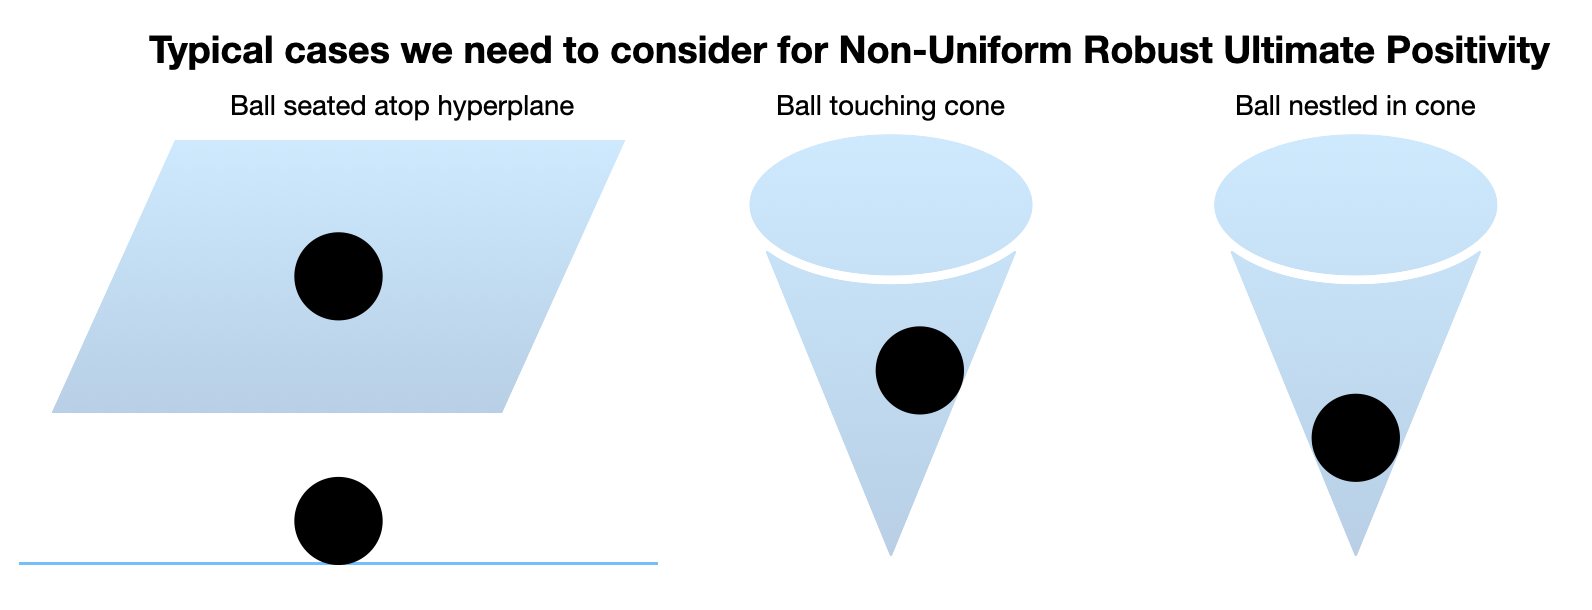
\includegraphics[width=\textwidth]{picture1.png}
\caption{Visual intuition}
\label{fig:geometricpicture}
\end{figure}
\subsection{Decidability at order three}
\label{section:decidability2}
In this section, we prove Theorem \ref{thm:decide2}. As before, the techniques naturally apply to lower orders, and we omit their explicit treatment. Recall equation \ref{eq:grouping} and the surrounding discussion:
\begin{equation}
u_n/n^d\rho^n = \begin{bmatrix}
{\color{red!70!black} \mathbf{q}_{dom}^T(n) } & \mathbf{q}_{res}^T(n)
\end{bmatrix}
\begin{bmatrix}
{\color{red!70!black} \mathbf{p}_{dom}} \\
\mathbf{p}_{res}
\end{bmatrix}
\end{equation}
The crucial first task is to check whether for all points $\mathbf{p'}$ in the neighbourhood, \\$\liminf_{n\in\naturals}\seq{\mathbf{q}_{dom}(n), \mathbf{p'}_{dom}} = \mu(\mathbf{p'}) \ge 0$. Although Ultimate Positivity is guaranteed for the points where the inequality is strict, the neighbourhood may intersect the critical region where $\mu = 0$. If there are no non-dominant terms, this is irrelevant; but otherwise decidability hinges on whether we can handle the intersection.

We make cases, based on the presence of a pair of complex conjugates among the dominant roots. If the dominant terms are all real, then $\seq{\mathbf{q}_{dom}(n), \mathbf{p'}_{dom}} \ge 0$ is the intersection of at most two halfspaces (of the form $z - |w| \ge 0$). The neighbourhood must lie entirely above the separating hyperplanes (ball atop hyperplane in Figure \ref{fig:geometricpicture}). The points where the neighbourhood is tangent to the planes have algebraic coordinates. The three polynomial equations for the three coordinates come from the facts that: (i) the point lies on the plane, (ii) the point lies on the surface of the neighbourhood, (iii) the gradient of $(\mathbf{p'} - \mathbf{p})^T\mathbf{M}(\mathbf{p'} - \mathbf{p})$ is along the normal to the plane. This gives us low-order, decidable instances of Ultimate Positivity.

Otherwise, there are no non-dominant terms, and $\seq{\mathbf{q}_{dom}(n), \mathbf{p'}_{dom}} = z + x\cos n\theta + y\sin n\theta$. We assume $\theta$ is not a rational multiple of $2\pi$ (can be detected, Theorem \ref{thm:abelian}): otherwise, the region where $\mu(\mathbf{p'}) \ge 0$ is again a finite union of halfspaces. Recall equation \ref{eq:liminfmin}. We get that $\mu(\mathbf{p'}) = z -\sqrt{x^2 + y^2}$. As shown in Figure \ref{fig:geometricpicture}, the critical region $\mu(\mathbf{p'})$ is a cone. Here, decidability follows by simply using Theorem \ref{thm:renegar} (Renegar) to evaluate the truth of this sentence in the First Order Theory of the Reals.
\begin{equation}
\label{eq:firsttask}
\chi := \forall \mathbf{p'}.~ (\mathbf{p'} - \mathbf{p})^T\mathbf{M}(\mathbf{p'} - \mathbf{p}) \le 1 \Rightarrow \mu(\mathbf{p'}) \ge 0
\end{equation}

\subsection{Hardness at order four}
\label{section:hardness2}
In this section, we prove Theorem \ref{thm:hardness2}. More precisely, given $t \in \mathcal{T}$, $0 < \rho < 1$, and a precision $\varepsilon > 0$, we will use the purported decidability of $\mathbf{S}$-Robust non-uniform Ultimate Positivity to approximate the maximal $\ell$ such that the set 
$$
E_{\ell\rho^n}(t) = \{s\in \reals: \ell\rho^n[nt - s] \le 1 \text{ for infinitely many } n\}
$$
is non-empty. We assume that $t$ is represented by an algebraic $p$, such that $\theta = 2\pi t = \arccos(p)$. The characteristic polynomial of our recurrence relation is $(X-1)(X-\nu)(X^2 - 2pX + 1)$, where $\nu = 1/\rho^2$. As in the previous reduction, we choose $\mathbf{S} = \frac{1}{2}(\mathbf{V}^{-1})^T\mathbf{V}^{-1}$ such that its translation $\mathbf{M}$ to the solution space is $1/2$ times the identity matrix. In the solution space, our neighbourhood is the ball of radius $\sqrt{2}$. We assume the solution to be $z + x\cos n\theta + y\sin n\theta + w\nu^n$.

We take the centre to be $(z = 2, x = 0, y= 0, w = -r), r > 0$. Observe that the neighbourhood intersects the cone $\mu = 0$ in the unit ring $z= 1, x^2 + y^2 = 1, w = -r$. This corresponds to the ball nestled in cone situation in Figure \ref{fig:geometricpicture}. The way to see this is by noting that the cone $z^2 = x^2 + y^2$ may be thought of as being carved by \textit{infinitely} many hyperplanes $z + x\cos \phi + y\sin \phi = 0$. The centre of the ball is at unit distance from each of them; going along the normal $(-1/\sqrt{2}, -\cos\phi/\sqrt{2}, -\sin\phi/\sqrt{2}, 0)$ for a distance of $\sqrt{2}$ gives the point of tangency $(1, -\cos\phi, -\sin\phi, -r)$. We need to crucially decide if Ultimate Positivity holds at \textit{each} of these points. 

This is not trivial: although Ultimate Positivity is known to be decidable for Simple LRS \cite{ouaknine2014ultimate}, as well as for low order LRS \cite{joeljames3}, the techniques therein assume that all input is algebraic, which is not the case here. Continuity arguments to interpolate from the decidable points likely don't work, as algebraic numbers form a measure $0$ countable subset of the uncountable reals.

Our problem is to decide whether, for each $\phi$, the inequality
\begin{equation}
\label{eq:ring}
1 -\cos(n\theta-\phi) \ge r\nu^n
\end{equation}
holds for all sufficiently large $n$. We reason exactly as we did in the previous section. Note $\nu = 1/\rho^2$, $[bx]_b = b[x]$, and the analogue of Lemma \ref{lemma:numerical}
\begin{lemma}
\label{lemma:numerical2}
For every $r, \varepsilon > 0$, we can compute $N$ such that,
$$1 - \cos x < r\nu^N  \Rightarrow 1- \cos x > (1 - \varepsilon)^2\frac{x^2}{2}$$
\end{lemma}

\textbf{Case YES}.
Since $\theta$ is not a rational multiple of $2\pi$, $n\theta - \phi$ can be a multiple of $2\pi$ at most once. We conclude that for every $\phi = 2\pi s$, $[n\theta-\phi]_{2\pi}^2 > 2r\nu^n$ for all sufficiently large $n$. In other words, for every $s$, $\left(\pi\sqrt{\frac{2}{r}}\right)\rho^n[nt - s] \le 1$ for only finitely many $n$. $\left(\pi\sqrt{\frac{2}{r}}\right)$ is thus an upper-bound for $\ell$.

\textbf{Case NO}.
There exists a $\phi_0$ such that $1 - \cos n\theta$ is infinitely often less than $r\nu^n$. Hence, for any $\varepsilon$, one can compute an $N$, and apply Lemma \ref{lemma:numerical2} on the infinitely many times $1 - \cos n\theta$ is small enough. We get that for every $\varepsilon$, there are infinitely many $n$, $(1-\varepsilon)^2[n\theta-\phi_0]_{2\pi}^2 < 2r\nu^n$. Since $\varepsilon$ is arbitrary, we can simplify as in the previous case, and argue that for $s_0$, $\left(\pi\sqrt{\frac{2}{r}}\right)\rho^n[nt - s_0] \le 1$ for infinitely many $n$. $\left(\pi\sqrt{\frac{2}{r}}\right)$ is thus a lower-bound for $\ell$.

